\documentclass[border=10pt]{standalone}
\usepackage{amsmath}
\usepackage{tikz}
\usetikzlibrary{shapes.geometric, arrows.meta, positioning, fit, calc, backgrounds}

\tikzset{
    block/.style={rectangle, draw, fill=blue!10, text width=5em, text centered, rounded corners, minimum height=3em},
    wideblock/.style={rectangle, draw, fill=blue!10, text width=8em, text centered, rounded corners, minimum height=3em},
    envblock/.style={rectangle, draw, fill=green!10, text width=6em, text centered, rounded corners, minimum height=3em},
    netblock/.style={rectangle, draw, fill=orange!10, text width=7em, text centered, rounded corners, minimum height=4em},
    lossblock/.style={rectangle, draw, fill=red!10, text width=6em, text centered, rounded corners, minimum height=3em},
    datablock/.style={rectangle, draw, fill=yellow!10, text width=7em, text centered, rounded corners, minimum height=2.5em},
    arrow/.style={-{Stealth[length=3mm]}, thick},
    dashedarrow/.style={-{Stealth[length=3mm]}, thick, dashed},
    gradient/.style={-{Stealth[length=3mm]}, thick, red},
}

\begin{document}
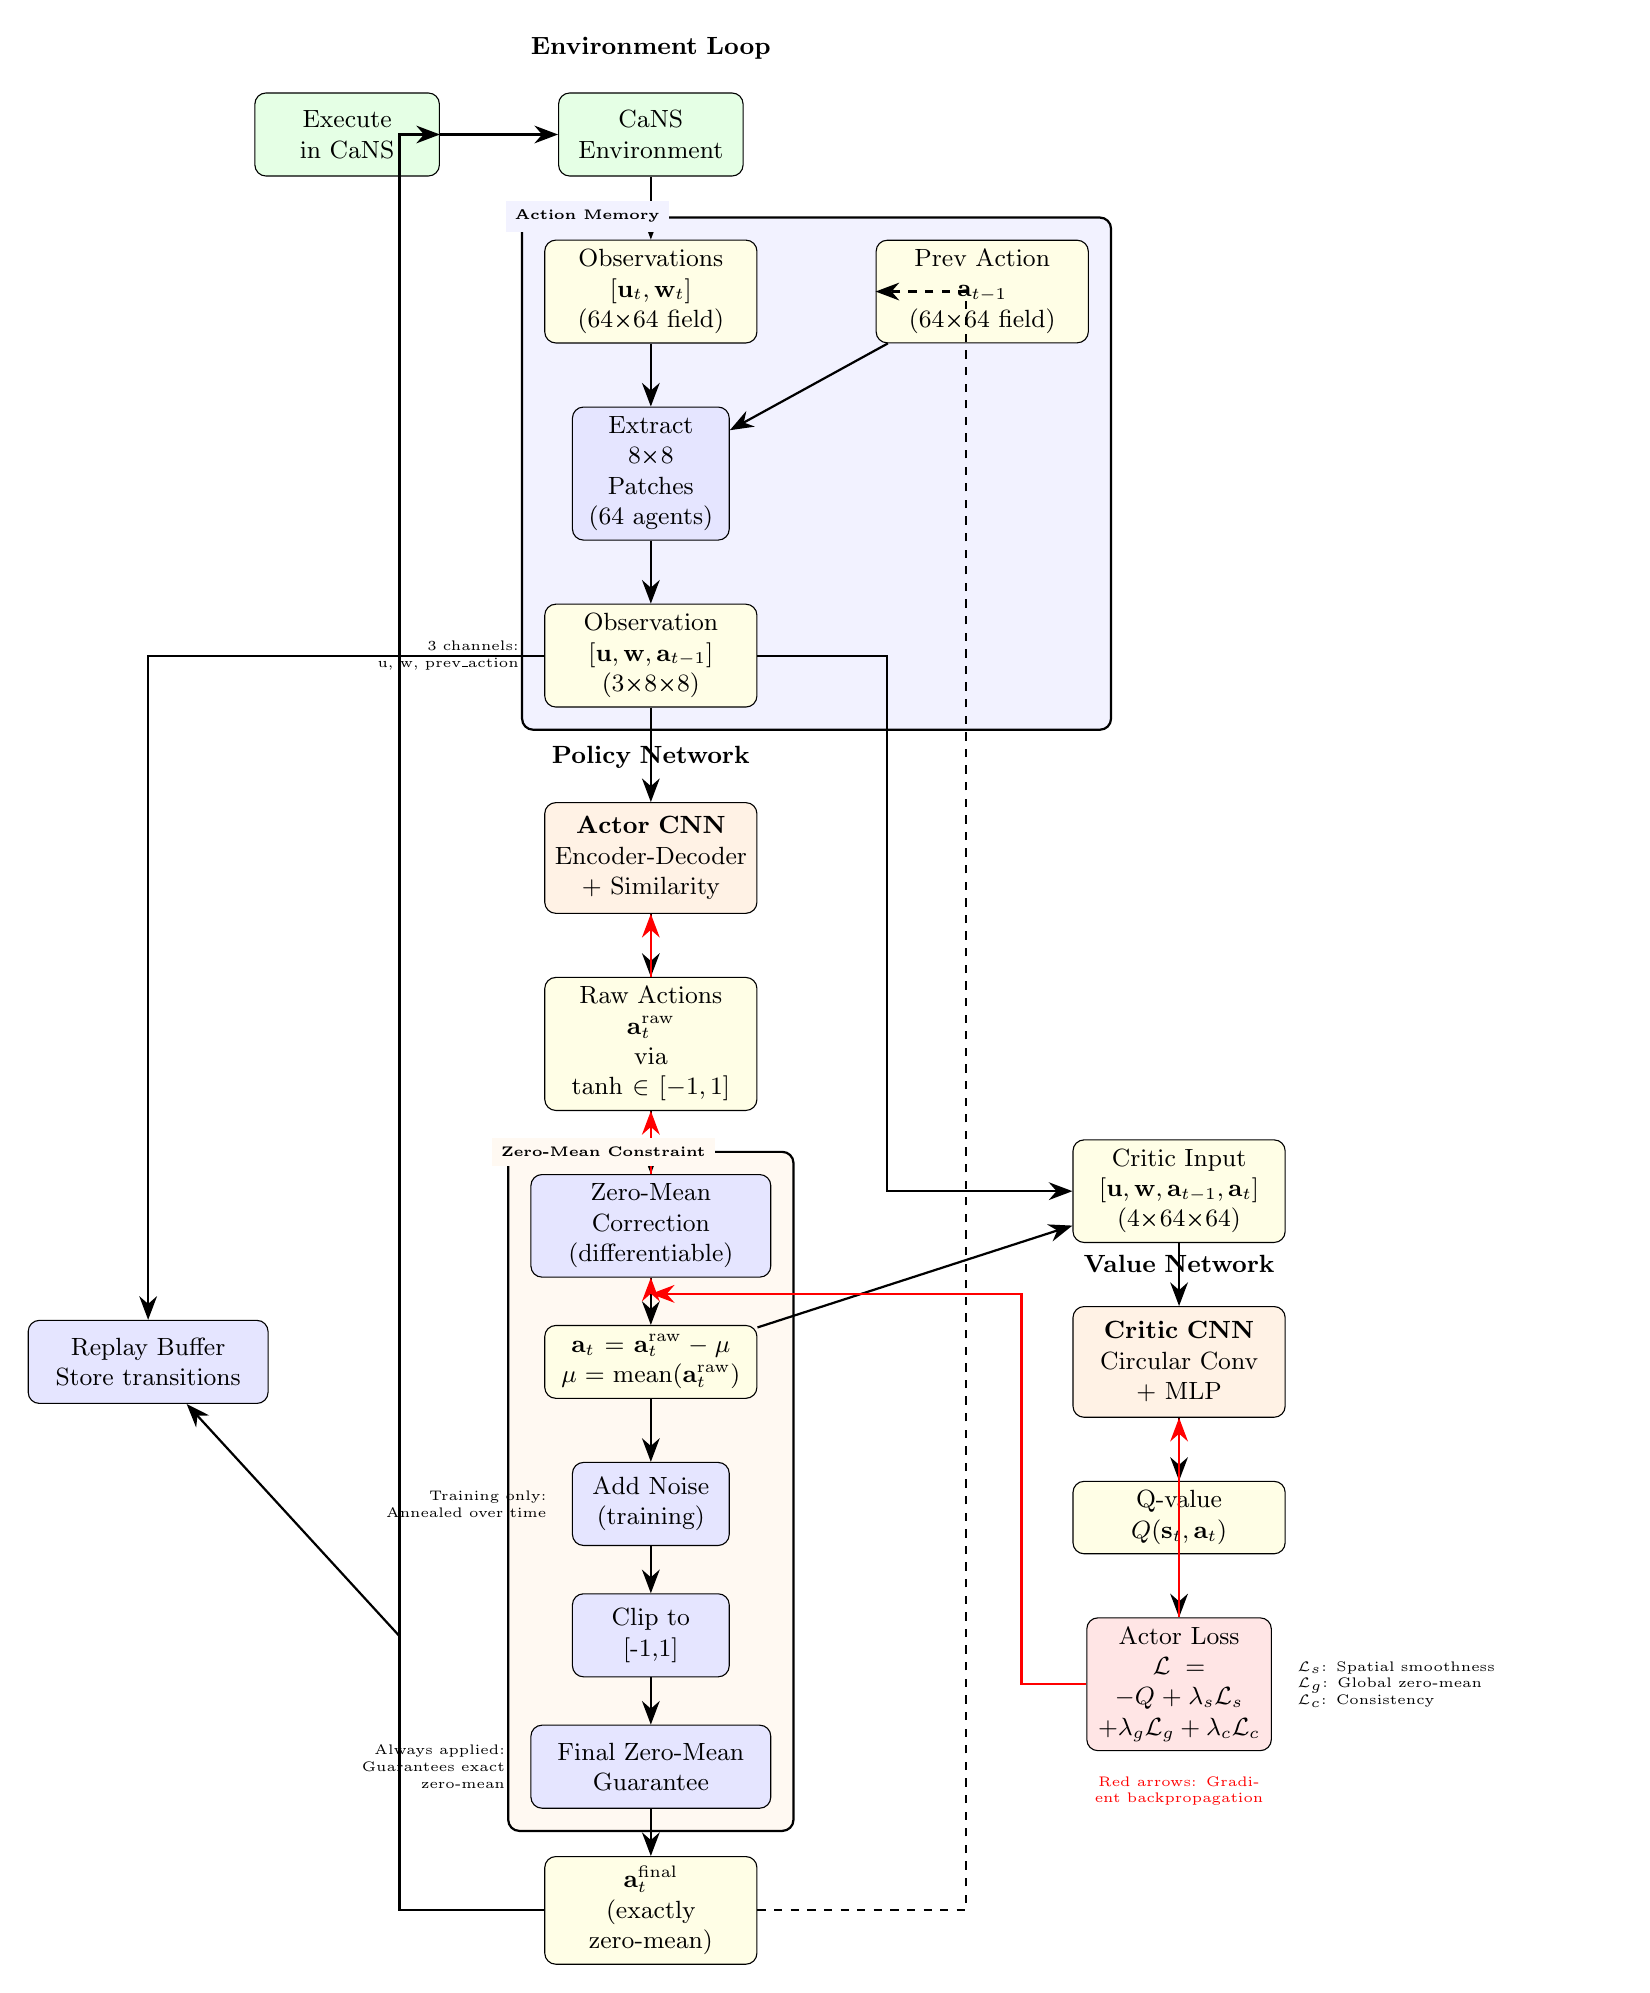
\begin{tikzpicture}[node distance=1.2cm, font=\small]

% Environment
\node[envblock] (env) {CaNS\\Environment};
\node[datablock, below=0.8cm of env] (obs) {Observations\\$[\mathbf{u}_t, \mathbf{w}_t]$\\(64×64 field)};

% Previous action storage
\node[datablock, right=1.5cm of obs] (prevact) {Prev Action\\$\mathbf{a}_{t-1}$\\(64×64 field)};

% Patch extraction
\node[block, below=0.8cm of obs] (patch) {Extract\\8×8 Patches\\(64 agents)};
\node[datablock, below=0.8cm of patch] (obs3ch) {Observation\\$[\mathbf{u}, \mathbf{w}, \mathbf{a}_{t-1}]$\\(3×8×8)};

% Actor Network
\node[netblock, below=1.2cm of obs3ch] (actor) {\textbf{Actor CNN}\\Encoder-Decoder\\+ Similarity};
\node[datablock, below=0.8cm of actor] (actraw) {Raw Actions\\$\mathbf{a}^{\text{raw}}_t$\\via $\tanh \in [-1,1]$};

% Zero-mean correction
\node[wideblock, below=0.8cm of actraw] (zeromean) {Zero-Mean\\Correction\\(differentiable)};
\node[datablock, below=0.6cm of zeromean] (actcorr) {$\mathbf{a}_t = \mathbf{a}^{\text{raw}}_t - \mu$\\$\mu = \text{mean}(\mathbf{a}^{\text{raw}}_t)$};

% Noise and clipping (training only)
\node[block, below=0.8cm of actcorr] (noise) {Add Noise\\(training)};
\node[block, below=0.6cm of noise] (clip) {Clip to [-1,1]};
\node[wideblock, below=0.6cm of clip] (finalmean) {Final Zero-Mean\\Guarantee};
\node[datablock, below=0.6cm of finalmean] (actfinal) {$\mathbf{a}^{\text{final}}_t$\\(exactly zero-mean)};

% Critic Network (on the right side)
\node[netblock, right=4cm of actcorr] (critic) {\textbf{Critic CNN}\\Circular Conv\\+ MLP};
\node[datablock, above=0.8cm of critic] (criticinput) {Critic Input\\$[\mathbf{u}, \mathbf{w}, \mathbf{a}_{t-1}, \mathbf{a}_t]$\\(4×64×64)};
\node[datablock, below=0.8cm of critic] (qvalue) {Q-value\\$Q(\mathbf{s}_t, \mathbf{a}_t)$};

% Loss computation
\node[lossblock, below=0.8cm of qvalue] (actorloss) {Actor Loss\\$\mathcal{L} = -Q + \lambda_s \mathcal{L}_s$\\$+ \lambda_g \mathcal{L}_g + \lambda_c \mathcal{L}_c$};

% Replay buffer (left side)
\node[wideblock, left=3.5cm of actcorr] (buffer) {Replay Buffer\\Store transitions};

% Back to environment
\node[envblock, left=1.5cm of env] (execute) {Execute\\in CaNS};

% Draw arrows - Forward pass
\draw[arrow] (env) -- (obs);
\draw[arrow] (obs) -- (patch);
\draw[arrow] (prevact) -- (patch);
\draw[arrow] (patch) -- (obs3ch);
\draw[arrow] (obs3ch) -- (actor);
\draw[arrow] (actor) -- (actraw);
\draw[arrow] (actraw) -- (zeromean);
\draw[arrow] (zeromean) -- (actcorr);
\draw[arrow] (actcorr) -- (noise);
\draw[arrow] (noise) -- (clip);
\draw[arrow] (clip) -- (finalmean);
\draw[arrow] (finalmean) -- (actfinal);

% Actions to environment
\draw[arrow] (actfinal) -| ($(actfinal)!0.5!(buffer)$) |- (execute);
\draw[arrow] (execute) -- (env);

% Actions to replay buffer
\draw[arrow] ($(actfinal)!0.5!(buffer)$) -- (buffer);
\draw[arrow] (obs3ch) -| (buffer);

% Critic input preparation
\draw[arrow] (obs3ch) -- ++(3,0) |- (criticinput);
\draw[arrow] (actcorr) -- (criticinput);
\draw[arrow] (criticinput) -- (critic);
\draw[arrow] (critic) -- (qvalue);
\draw[arrow] (qvalue) -- (actorloss);

% Gradient flow (red dashed)
\draw[gradient] (actorloss) -- ++(0,1) -| (critic);
\draw[gradient] (actorloss) -- ++(-2,0) |- ($(actcorr)!0.5!(zeromean)$);
\draw[gradient] ($(actcorr)!0.5!(zeromean)$) -- (zeromean);
\draw[gradient] (zeromean) -- (actraw);
\draw[gradient] (actraw) -- (actor);

% Store prev_action
\draw[dashedarrow] (actfinal) -- ++(4,0) |- (prevact);

% Annotations
\node[above=0.3cm of env, text width=6cm, align=center] {\textbf{Environment Loop}};
\node[above=0.3cm of actor, text width=5cm, align=center] {\textbf{Policy Network}};
\node[above=0.3cm of critic, text width=5cm, align=center] {\textbf{Value Network}};

% Loss components annotation
\node[right=0.2cm of actorloss, text width=4cm, font=\tiny, align=left] {
    $\mathcal{L}_s$: Spatial smoothness\\
    $\mathcal{L}_g$: Global zero-mean\\
    $\mathcal{L}_c$: Consistency
};

% Channel annotation
\node[left=0.2cm of obs3ch, text width=3cm, font=\tiny, align=right] {
    3 channels:\\
    u, w, prev\_action
};

% Training vs inference note
\node[left=0.2cm of noise, text width=3cm, font=\tiny, align=right] {
    Training only:\\
    Annealed over time
};

\node[left=0.2cm of finalmean, text width=3cm, font=\tiny, align=right] {
    Always applied:\\
    Guarantees exact\\
    zero-mean
};

% Gradient flow annotation
\node[below=0.2cm of actorloss, text width=4cm, font=\tiny, align=center, text=red] {
    Red arrows: Gradient backpropagation
};

% Key insight box
\begin{scope}[on background layer]
\node[draw, fill=blue!5, thick, rounded corners, fit={(obs3ch) (prevact)}, inner sep=8pt] (actionmemory) {};
\end{scope}
\node[above right=-0.2cm and -0.2cm of actionmemory.north west, fill=blue!5, font=\tiny\bfseries] {Action Memory};

\begin{scope}[on background layer]
\node[draw, fill=orange!5, thick, rounded corners, fit={(zeromean) (actcorr) (finalmean)}, inner sep=8pt] (zeroconstraint) {};
\end{scope}
\node[above right=-0.2cm and -0.2cm of zeroconstraint.north west, fill=orange!5, font=\tiny\bfseries] {Zero-Mean Constraint};

\end{tikzpicture}
\end{document}
